%!TEX encoding = UTF-8 Unicode
%!TEX program = xelatex

\documentclass[bachelor]{ustcthesis}
% bachelor|master|doctor
\usepackage{ustcextra}
\graphicspath{{figures/}}
\bibliographystyle{ustcauthoryear}
% \bibliographystyle{ustcnumerical}


\newcommand{\docname}{软件工程即时通信系统}
\renewpagestyle{front}[\zihao{-5}]{
    \sethead{}{\docname 需求规格说明书}{}
    \setfoot{}{\thepage}{}
    \headrule
}
\renewpagestyle{main}[\zihao{-5}]{
    \sethead{}{\docname 需求规格说明书}{}
    \setfoot{}{\thepage}{}
    \headrule
}
\newcommand{\HRule}{\rule{\linewidth}{0.5mm}}

\begin{document}



\begin{titlepage}
\begin{center}
~\\[5cm]
\HRule \\[0.4cm]
{\huge \bfseries \docname\\需求规格说明书}\\[0.4cm]
\HRule \\[1.5cm]

\begin{tabular}{ccc}
  & 人员 & 日期 \\ 
拟制 & 王嵩超\ 罗炳琨\ 龚正\ 周智维 & 2018-04-23 \\ 
评审人 & 罗炳琨\ 周智维 & 2018-04-25 \\ 
批准 & 王嵩超& 2018-04-28 \\ 
签发 & 王嵩超& 2018-04-29 \\ 
\end{tabular} 

\end{center}
\end{titlepage}



\frontmatter
\begin{abstract}
本文是软件工程13组的需求规格说明书,其模板修改自于中国科学技术大学本硕博毕业论文 \LaTeX{} 模板示例文件,该模板由
zepinglee和seisman创建,遵循中国科学技术大学的论文写作规范,适用于撰写学士、硕士和博士学位论文。

\keywords{软件工程\zhspace{} 中国科学技术大学\zhspace{} 学位论文\zhspace{} \LaTeX{}~通用模板\zhspace{} 学士\zhspace{}
硕士\zhspace{} 博士\zhspace{} 示例文档\zhspace{} 模板说明文档}

% \begin{table}[htbp]
% \centering
% \caption{缩略词清单} \label{tab:abbr}
% \begin{tabular}{|c|c|c|}
%     \hline
%     缩略语 & 英文全名 & 中文解释 \\
%     \hline
%     c & d & e\\
%     \hline
% \end{tabular}
% \end{table}

\end{abstract}

\tableofcontents
\listoffigures
\listoftables
% \listofalgorithms  % 算法索引,如不需要,可直接注释掉本行
% \begin{notation}

%\centering
%XX 软件需求规格说明书

%关键词:能够体现文档描述内容主要方面的词汇。
 
%摘要:


\centering
\begin{tabular}{rl}
$\ln x$ & natural logarithm $\log_ex$ \\
$\log x$ & common logarithm $\log_{10}x$ \\
$x\ \mathrm{mod}\ y$ & remainder \\
\end{tabular}

\end{notation}


\mainmatter
\chapter{简介}
\section{目的}
%This section should state the purpose of the document. It could also specify the intended audience. Identify the product whose software requirements are specified in this document.

%这部分要描述文档的目的。应该指明读者。说明本需求文档描述了哪个产品的软件需求。

本文档为软件工程课程实验二即时通讯系统的需求说明文档。编写该本文档的主要目的是对即时通讯系统的软件需求进行说明,为该系统的详细设计、开发工作提供依据,为项目设计人员、开发人员、使用人员和其他相关人员对系统实现的功能达成统一的认识提供一个明确的书面说明。

本文档的主要读者为项目设计人员,软件开发、测试人员,指导人员,以及目标用户等。

\section{范围}
% This section should address areas which this document includes and that are specifically excludes. 

% 本节应描述文档所包括和不包括的内容。
本文档包括了以需求为中心的相关要求,包括产品所处在的运行环境,所有的功能需求,性能需求,质量特性。
\linebreak
本文档不包括产品的开发、实现等细节内容。

\chapter{总体概述}

%Describes the general elements that may affect the product and the requirements on the product. It includes the following four parts. Note that this section should not describe the specific requirements, instead, it makes the specific requirements to be described more understandable.

%本节描述影响产品和产品需求的一般因素。由以下4个部分构成。 有一点需说明的是本节不描述具体的需求,只是使那些将要描述的具体需求更易于理解。
\section{软件概述}
\subsection{项目介绍}
%Describe the context and origin of the project being specified in this SRS. For example, state whether this project is a follow-on member of a project family, a replacement for certain existing systems, or a new, self-contained project.

%描述本软件需求所描述的项目的背景。例如:本项目是一系列版本中的一个,或者是替代某个已经存在的系统,还是一个新的独立的项目。

本项目要开发的软件为一个独立的即时通讯系统,为软件工程课程实验二的选题之一。

\subsection{产品环境介绍}
%Describes the whole environment that is composed of this software and other products / projects.
%\begin{itemize}
%\item If this software is independent or fully self-contained, state it here.
%\begin{itemize}
%\item describe the function of each component of that larger system/project, and identify the interfaces.
%\item determine the main external interfaces of this software.( Note: Do not describe the interfaces in detail; the detailed description will be provided in other part of the SRS document.)
%\item describe related hardware of the product and peripheral equipment.( Note: This is only  a general description, not in detail.)
%\end{itemize}
%\end{itemize}

%It is very helpful to describe the main components, interconnection and external interfaces of the larger system/project by Block Diagram. This part should not provide a detailed design solution, or detailed design constraint for the solution (the detailed design constraint will be described in the section of specific requirement). This section is the basis of the design constraints.

%描述的是本产品与其它产品或项目所组成的整体环境。

%1.如果本产品是独立的并完全自我包含,在此说明这一点。

%2.如果SRS定义的产品是更大的系统或项目的组件(此种情形经常发生),那么应:

%	A. 描述此大系统或项目每个组件的功能,并且标识接口。
%
%	B.  确定本软件产品主要外部接口。( 注意:在此部分并不进行这些接口的详细描述;对这些接口的详细描述在SRS的其它 部分提供。)
%    
%    C. 描述相关产品硬件和所使用的外部设备。(  注意:  这只是概述性描述。)
%
%通过方块图来描述大系统或项目的主要组件,互连性以及外部接口将是非常有帮助的。本部分不应提出一个具体的设计解决方案或对解决方案的具体设计约束(具体设计约束将在具体需求章节中描述)。本部分内容是产生设计约束的基础。

本系统最终产品将分为服务端和客户端两大组件。
服务端运行于linux或windows平台上,为客户端提供服务。
客户端运行于linux,windows,android,ios等平台上,为用户提供操作接口。

\section{软件功能}
%Summarizes the major functions that must be implemented through the software, and the functions to be implemented through user operation. Details will be provided in the Specific Requirement, so only a summary (such as a directory list) is needed here. The functions should be organized to make them understandable to the readers, and be appropriate for subsequent design and tests. Diagrams like top-level data flow diagram or object class diagram are recommended to illustrate the relationships among the major requirement groups 
%
%Sometimes, this section can directly refer to the superior specification of the software that allocate the specific requirements to this software ( if existed ).
%The specific requirements should not be described in this section. But this section is the basis of the specific requirements.
%
%概述软件的必须实现的和通过用户操作实现的主要功能。这里只需要进行简要描述(例如目录列表),详细描述在详细需求部分描述。对需求功能进行组织,以便于读者理解,并能指导后续的设计和测试。可以用图表来表示主要需求群组之间的关系,例如:高层的数据流图,面向对象的分析等。
%
%有时此部分所要求的功能概述可以从分配具体功能给此软件产品的更高层规格(如果存在的话)直接引用。
%
%本节不应描述具体需求。但本节内容是具体需求章节的基础。
\begin{itemize}
\item 一对一即时通讯
\item 群聊
\item 语音通话
\item 视频通话
\item 用户配对
\item 表情包管理
\end{itemize}

\section{用户特征}
%List down the basic required characteristics of the user or operator of the system. E.g. the experience, Skill level, required role etc., 
%This part should not describe the specific requirements, instead, it provides the basis for the specific requirements.
%
%列出对用户或系统操作者的要求,如:经验,能力,角色等。
%
%本节不应描述具体需求。但本节内容是具体需求章节的基础。

本系统分为服务端和客户端两大组件。

服务端的主要使用者为有搭建即时通讯系统需求的用户,要求具备一定的计算机知识和运维经验。

客户端的主要使用者为有即时通讯需求的用户,用户无需具备特殊的专业知识,但要求具有一定的计算机使用知识。

\section{假设和依赖关系}
List any assumed factors (as opposed to known facts) that could affect the requirements stated in the SRS. These could include third party or commercial components that you plan to use, issues around the development or operating environment, or constraints. The project could be affected if these assumptions are incorrect, are not shared, or change. Also identify any dependencies the project has on external factors, such as software components that you intend to reuse from another project, unless they are already documented elsewhere (for example, in the vision and scope document or the project plan). 

列出可能影响SRS中需求的所有的假设因素(与已知事实相对而言),包括准备使用的第三方或商业组件,操作和开发环境的问题约束等。如果上述假设不正确、没有被告知或者改变了都将对项目产生影响。列出项目对外部条件的依赖,例如重用其他项目的模块等。如果在其他文档(例如项目计划或范围文档等)里已经描述了,在这里可以不用描述。

\chapter{具体需求}
% <The following sections must be repeated for each requirement. >

% 在每一条需求描述中重复下列部分
\section{功能需求}
% This section describes how the input of the software is translated to the output. It describes the essential action the software must perform.

% For each kind of function, or each independent function in some cases, the requirements of input, process and output must be described, which are usually organized with the following four subsections:

% 本子章节应描述软件产品的输入怎样被转换成输出。它描述了软件必须执行的基本动作。 

% 对每一类功能或有时对每一个单独的功能,必须描述输入、处理、输出方面的需求。这些通常以下面四个子段落来组织:
% \subsection{功能需求1}
% Please don't use "Functional Requirement(1)" as the title of the functional requirement. Name the functional requirements with a few simple words and a requirement ID.  For example:
% 
% R.INTF.CALC.001 Calculating expression
% 
% R.INTF.CALC.002 Print
% 
% Naming the requirement ID shall follow the Software Requirements Management Procedure (REP01)
% 
% 用需求编号加上简短词汇做为功能需求名,不要用“功能需求(1)”作为功能名,例如:R.INTF.CALC.001 计算表达式
% 
% R.INTF.CALC.002 打印
% 
% 需求编号规则按照软件需求管理规程(REP01)进行
% \subsubsection{介绍}
% <Itemize the detailed functional requirements associated with this feature. These are the software capabilities that must be present in order for the user to carry out the services provided by the feature.  Include how the project should respond to anticipated error conditions or invalid inputs. Requirements should be concise, complete, unambiguous, verifiable, and necessary. Use "TBD" as a placeholder to indicate when necessary information is not yet available. >
% 
% 逐条列出与本特性相关的功能需求。包括项目如何响应预期的错误输入,非法条件和无效输入。需求应该简明,完整,不含糊,可验证,必要的。 当需要的信息不确定的时候使用“待定”。
% \subsubsection{输入}
% This section consists of:
% A. Detailed description of all input data of the function, including:
% Source of input
% Quantify
% Measurement units
% Timing requirements
% Valid input range that contains the precision and tolerance
% B. Reference of interface specification or interface control document that are provided in proper place.
% 
% 本子段落应包含下列内容:
% 
% A. 对该功能所有输入数据的详细描述,包括:
% 
% 		输入来源
% 		数量
% 		度量单位
% 		时间要求
% 		包含精度和容忍度的有效输入范围
% 		
% B. 在适当的地方提供的对接口规格或接口控制文档的参考。
% \subsubsection{处理}
% Describes all the operations on the input data, and the process to get the output data, including the following specifications:
% A. Verification of input data
% B. Exact order of the operations, including the time sequene of each event.
% C. Response to exception, such as:
% 		 Overflow
% 		Communication failure
% 		Error process
% D. Any method used to transfer the input data to the output data. (such as equation,mathematic algorithm and logical operation)
% For example.
% 		The formula to calculate the income tax in a pay roll.
% 		the weather model used for weather forecast
% E. Verification of output data.
% 本子段落应描述对输入数据所执行的所有操作和如何获得输出的过程。这包括下列规格:
% 
% A. 输入数据的有效性检测。
% 
% B. 操作的确切次序,包括各事件的时序。
% 
% C. 对异常情况的回应,例如:
% 		溢出
% 		通信失败
% 		错误处理
% D. 用于把系统输入转换到相应输出的任何方法(诸如方程式,数学算法,逻辑操作)。例如,这可能描述下列方面:
% 		对工资单里代扣所得税的计算公式。
% 		用于气象预报的气象模型。
% 		
% E.	对输出数据的有效性检测。
% \subsubsection{输出}
% This section should include:
% A. The detailed description of output data of the function, including:
% 		Target to output to (Such as a printer or a file)
% 		Quantity
% 		Measurement units
% 		Time sequence
% 		Valid output range including the precision and tolerance
% 		Process of the invalid value.
% 		Error message.
% B. Reference of interface specification or interface control document that are provided in proper place.
% For the systems with their requirements focused on the input/output actions, all the important input/output actions and the time sequences of the input/output pairs should be described in the SRS. In a system that inputs and actions are memorized as the basis for the reactions to be taken, the timing sequence for the input/output pairs must be available here. This kind of functional action is similar to a status machine.  
% 本子段落应包含:
% 
% A. 对该功能所有输出数据的详细描述,这个描述包括:
% 		输出的到何处(如打印机,文件)
% 		数量
% 		度量单位
% 		时序
% 		包含精确度和容忍度的有效输出范围
% 		对非法值的处理
% 		错误消息
% 		
% B. 在适当的地方提供对接口规格或接口控制文档的参考。
% 
% 此外,对那些需求集中在输入/输出行为的系统,SRS应描述所有重要的输入/输出行为及输入输出对的次序。对一个需要记忆其行为以根据输入和过去的行为进行反应的系统,输入输出对的次序是要求的;这种功能行为就类似于有限状态机。

\subsection{R.INSTANT.MESSAGE.USERS.001 新用户注册}
\subsubsection{介绍}

账号注册,用户使用邮箱和密码新建账号。每位用户在注册时需要提供基本的用户信息(用作用户ID的邮箱,密码),和可选的用户资料(User Profile,如头像,性别,出生日期,所在地等)。

\subsubsection{输入}
\begin{itemize}
	\item 邮箱:可以接收邮件的合法邮箱
	\item 密码:由数字字母和特殊字符组成,三者均须出现,且至少为8位
	\item 确认密码:确保和密码一致
	\item (可选)用户资料:头像,性别,出生日期,所在地
	\item (可选)权限配置信息:
		\begin{enumerate}	
		\item 用户资料中的每个条目对自己好友是否可见
		\item 用户资料中的每个条目对陌生人是否可见
		\item 能否通过地理位置信息搜索到自己
		\end{enumerate}
	\end{itemize}

\subsubsection{处理}
\begin{enumerate}
	\item 检查邮箱是否合法
	\item 检查邮箱是否已被注册
	\item 检查密码是否和确认密码一致
	\item 检查密码强度是否合理
	\item 若用户上传了头像图片,检查该图片大小符合服务器上传文件大小限制
	\item 检查用户填写的其他用户资料值是否合法
	\item 将新用户记录插入数据库
	\end{enumerate}
若存在至少一项检查未通过,则本次操作失败;若所有检查均通过,则在数据库用户表中插入一条新记录,并根据输入信息填写字段值。

\subsubsection{输出}
在用户界面提示注册成功或失败。对于失败的操作需要提示出错原因(如数据项不合法、网络异常)。


\subsection{R.INSTANT.MESSAGE.USERS.002 变更自己的用户资料(User Profile)}
\subsubsection{介绍}
应允许用户在创建自己的帐号后,再次修改自己的用户资料。\\
{
	\color{red}
	为用户的隐私考虑,用户可配置自己用户资料各个字段的访问权限,原则上应包括:
	\begin{itemize}
		\item 该项对好友是否可见
		\item 该项对陌生人是否可见
	\end{itemize}
	(用户ID由于会被多个数据库表所引用,修改开销较大,故修改用户ID未列入需求。)
}


\subsubsection{输入}
\begin{itemize}
	\item 要修改的用户资料
	\item (可选)用户资料各字段的权限配置信息
	\item 当前用户所对应的ID(由客户端程序获得,无需用户输入)
	\end{itemize}

\subsubsection{处理}
检查修改后的用户资料是否合法,与R.INSTANT.MESSAGE.USERS.001中的检查步骤相同。
若存在至少一项检查未通过,则本次操作失败;若所有检查均通过,则在数据库用户表中修改已存在的记录,并根据输入信息填写字段值。
\subsubsection{输出}
在用户界面提示修改成功或失败。对于失败的操作需要提示出错原因(如数据项不合法、网络异常)。


\subsection{R.INSTANT.MESSAGE.USERS.003 使用用户ID查找用户资料(User Profile)}
\subsubsection{介绍}
用户可通过搜索另一用户的ID来访问另一个用户所公开的基本资料。
\subsubsection{输入}
\begin{itemize}
	\item 要查询的用户ID
	\end{itemize}
\subsubsection{处理}
在数据库内执行查询语句,若查找到相应用户,则返回该用户{\color{red}设置为公开访问权限的}用户资料项;若未查找到,本次操作失败。
\subsubsection{输出}
若操作成功,在用户界面显示相应的用户资料;若操作失败,返回相应的出错原因(如用户不存在、网络异常)。


\subsection{R.INSTANT.MESSAGE.USERS.004 通过地理位置发现周边的用户}
\subsubsection{介绍}
通过GPS或基站信号记录每位用户的大致或精确的位置,由服务器完成分析,并向每位用户推送距离该用户较近的50个用户的用户资料。\\
{\color{red}为用户的隐私考虑,用户可选择是否公开自己的位置信息。若用户选择不公开位置信息,该用户将不会被返回至搜索结果。}
\subsubsection{输入(由客户端自动完成)}
\begin{itemize}
	\item 用户ID
	\item 用户的位置信息(由客户端通过系统API获取)
\end{itemize}
\subsubsection{处理}
服务器端采用聚类算法,将处于相近地理位置的用户聚集至相同的一组,并将该组用户推送给组内的每一个用户。
\subsubsection{输出}
在每个用户的推送中显示与其距离相近的用户列表,及其用户资料。


\subsection{R.INSTANT.MESSAGE.USERS.005 申请好友}
\subsubsection{介绍}
用户均可以通过以上各种搜索和发现用户的方式,向别的用户发出添加好友的请求。合法的申请发出后,对方若同意申请,则双方的联系人列表中均会加入对方的条目。
\subsubsection{输入}
\begin{itemize}
	\item 对方用户ID(当用户通过搜索或别的方式查找到某一用户并申请好友时,此字段由客户端自动获得)
	\item 一段文本验证消息
\end{itemize}
\subsubsection{处理}
\begin{itemize}
	\item 当用户发出申请后,此申请会作为一条文本消息发送至对方。文本消息发送时的处理流程见“R.INSTANT.MESSAGE.CHAT.001 文本聊天”。
	\item 对方接收到该消息后,可选择同意申请或者拒绝申请。若对方忽略该消息足够长时间,系统默认会选择拒绝申请。
	\item 当对方同意申请后,检测两个用户已有的好友数量。若至少有一个用户的已有好友数量到达允许的最大值,则本次操作失败并返回;
	若两个用户的已有好友数量均未到达最大值,则在各自的联系人表中加入对方的记录。
\end{itemize}
\subsubsection{输出}
\begin{itemize}
	\item 当用户发出合法的申请后,在用户界面显示“请求已发送,等待对方审核”的提示消息。
	\item 当对方对申请给出回复后,在用户界面显示相应的提示。
	\item 当操作失败时(好友数量过多,或网络原因),在用户界面显示出错原因。
\end{itemize}

{
\color{red}
\subsection{R.INSTANT.MESSAGE.USERS.006 好友删除}
\subsubsection{介绍}
用户可以在客户端将自己的好友删除
\subsubsection{输入}
\begin{itemize}
	\item 对方用户ID
\end{itemize}
\subsubsection{处理}
客户端向用户再次确认后,会向服务器发送请求,服务器会将对应的记录从数据库上删除。
\subsubsection{输出}
\begin{itemize}
	\item 当操作成功时,在用户界面显示成功提示
	\item 当操作失败时(好友不存在,或网络原因),在用户界面显示出错原因。
\end{itemize}
\subsection{R.INSTANT.MESSAGE.USERS.007 好友推荐}
\subsubsection{介绍}
由服务端依据多个维度的数据定期推送可能认识的人至用户客户端。可从以下的多个维度查找合适的候选用户用于推送:
\begin{itemize}
	\item 与该用户处于相同城市的用户
	\item 与该用户有着类似的用户资料字段(如年龄、兴趣爱好)
	\item 与该用户同时处于多个聊天群组
	\item 与该用户同时与多个另外的用户是好友关系(即二度人脉)
\end{itemize}
\subsubsection{输入}
由服务端自动推送,无需用户输入。
\subsubsection{处理}
当服务器计算出可能认识的用户时,向客户端发送推送消息。客户端发出通知,并生成一个用户列表,每一个条目均包含一个申请好友的入口。
\subsubsection{输出}
\begin{itemize}
	\item 当服务器计算出可能认识的用户时,客户端显示推送消息,以及申请好友的入口。
	\item 当服务器未筛选出符合条件的用户时,客户度静默失败,不显示任何推送。
\end{itemize}

\subsection{R.INSTANT.MESSAGE.USERS.008 用户主页}
\subsubsection{介绍}
每位注册用户均可拥有该用户专属的灵活的、高度自定义的个人主页。\\
主页本质上为HTML静态网页,用户可从本地上传多个HTML/CSS文档或者JavaScript脚本来定制他们的主页。此外,考虑到广大用户的方便,客户端本身也应提供基本的网页模板和相应的生成、部署工具。\\
用户可配置该主页的访问权限,原则上应可选以下选项:
\begin{itemize}
	\item 允许Internet用户访问
	\item 仅允许用户好友访问
	\item 仅允许用户指定的好友访问
	\item 仅允许用户自己访问
\end{itemize}


\subsection{R.INSTANT.MESSAGE.USERS.009 好友清理}
\subsubsection{介绍}
客户端可依据各种不同的筛选条件,如最近的聊天时间、聊天频率等,筛选出部分不常联系的好友。用户可在筛选出的列表中实施部分或批量删除。
\subsubsection{输入}
由系统生成,无需用户输入。
\subsubsection{处理}
客户端会向服务器发送请求,服务器会将对应的多条记录从数据库上删除
\subsubsection{输出}
\begin{itemize}
	\item 当操作成功时,在用户界面显示成功提示
	\item 当操作失败时(好友不存在,或网络原因),在用户界面显示出错原因。
\end{itemize}

\subsection{R.INSTANT.MESSAGE.USERS.0010 设置黑名单}
\subsubsection{介绍}
用户可以在客户端将其他用户加入黑名单,黑名单中的用户不能再向自己申请好友,发起临时会话。
\subsubsection{输入}
\begin{itemize}
	\item 对方用户ID
\end{itemize}
\subsubsection{处理}
客户端会向服务器发送请求,服务器会在数据库上增加黑名单的记录
\subsubsection{输出}
\begin{itemize}
	\item 当操作成功时,在用户界面显示成功提示
	\item 当操作失败时(用户不存在,或网络原因),在用户界面显示出错原因。
\end{itemize}

\subsection{R.INSTANT.MESSAGE.USERS.0011 隐私设置}
\subsubsection{介绍}
用户可以在客户端进行设置,可设置能够通过何种方式添加好友,好友可以查看那些资料,陌生人可以查看那些资料,主页查看权限等
\subsubsection{输入}
\begin{itemize}
	\item 添加好友方式
	\item 好友权限
	\item 陌生人权限
\end{itemize}
\subsubsection{处理}
客户端会向服务器发送请求,服务器从表单中读取数据,并在数据库上修改对应的记录
\subsubsection{输出}
\begin{itemize}
	\item 当操作成功时,在用户界面显示成功提示。
	\item 当操作失败时,在用户界面显示出错原因。
\end{itemize}
}


\subsection{R.INSTANT.MESSAGE.CHAT.001 发送文本消息}
\subsubsection{介绍}
发送文本给指定用户

\subsubsection{输入}
\begin{itemize}
	\item 文本消息
	\item 目标用户ID或群组ID
\end{itemize}

\subsubsection{处理}
\begin{enumerate}
	\item 检查文本长度是否超出限制,如果超出限制,则本次操作失败。
	\item 将消息发送给指定用户或群组

	\end{enumerate}

\subsubsection{输出}
\begin{itemize}
	\item 若发送成功,在聊天界面显示消息。
	\item 若发送失败,仍在聊天界面显示消息,外加发送失败的标志和出错原因,并显示重试操作按钮。
	\end{itemize}
	

\subsection{R.INSTANT.MESSAGE.CHAT.002 发送语音消息}
\subsubsection{介绍}
用户可使用设备自带的录音功能录制一段语音消息,并发送至对方用户或群组。
\subsubsection{输入}
用户语音
\subsubsection{处理}
\begin{enumerate}
	\item 检查音频大小是否超出限制,如果超出限制,则本次操作失败。
	\item 将音频文件发送给指定用户
	\end{enumerate}
\subsubsection{输出}
\begin{itemize}
	\item 若发送成功,在聊天界面显示。
	\item 若发送失败,仍在聊天界面显示,外加发送失败的标志和出错原因,并显示重试操作按钮。
	\end{itemize}

	
\subsection{R.INSTANT.MESSAGE.CHAT.003 发送图片消息}
\subsubsection{介绍}
用户可向对方用户或群组发送包含图片的消息。图片的来源可以是本机、网络或客户端的收藏夹。

\subsection{R.INSTANT.MESSAGE.CHAT.004 创建聊天群组}
\subsubsection{介绍}
创建一个新的聊天群组
\subsubsection{输入}
\begin{itemize}
	\item 群组名称
	\item 群组介绍文字
\end{itemize}
\subsubsection{处理}
\begin{enumerate}
	\item 检查群组名称字符串是否合法
	\item 检查该用户所创建群的数量是否已达上限
	\item 检查群组介绍文字是否符合长度要求
\end{enumerate}
若检查出错,则本次操作失败。若检查成功,则在数据库中创建相应的群组条目,并返回其唯一的数字ID。
\subsubsection{输出}
\begin{itemize}
	\item 若操作成功,则在用户界面显示新创建的群聊ID
	\item 若操作失败(名称不合法,群数量上限等原因),在用户界面显示出错原因
\end{itemize}

\subsection{R.INSTANT.MESSAGE.CHAT.005 邀请用户加入聊天群组}
\subsubsection{介绍}
邀请一个用户加入一个聊天群组,被邀请用户须是用户的好友。
\subsubsection{输入}
\begin{itemize}
	\item 被邀请的用户ID
	\item 群组ID(由客户端获取,用户无需输入)
\end{itemize}
\subsubsection{处理}
\begin{enumerate}
	\item 检测该群组已有的用户数量,若已达到最大值,则本次操作失败并返回。
	\item 检查用户ID、群组ID有效性。
	\item 检查被邀请用户是否是邀请者的好友。
	\item 若所有检查均通过,将邀请消息发送至被邀请的用户。否则本次操作失败。
	\item 对方接收到该邀请后,可选择同意邀请或者拒绝邀请。若对方忽略该消息足够长时间,系统默认会选择拒绝邀请。
	\item 将邀请结果回复给原用户。
\end{enumerate}
\subsubsection{输出}
\begin{itemize}
	\item 当用户发出合法的邀请后,在用户界面显示“请求已发送,等待对方审核”的提示消息。
	\item 当对方对邀请给出回复后,在用户界面显示相应的提示。
	\item 当操作失败时(好友数量过多,或网络原因),在用户界面显示出错原因。
\end{itemize}

\subsection{R.INSTANT.MESSAGE.CHAT.006 退出聊天群组}
\subsubsection{介绍}
解除用户与某聊天群组的关系。若该用户为群主,则用户在退出前须指定另一个成员作为新群主。
\subsubsection{输入}
群组ID(由客户端获取,用户无需输入)
\subsubsection{处理}
\begin{enumerate}
	\item 检查该用户是否为群主,如果是,则指引完成新群主的分配工作。
	\item 在数据库中执行相应的删除操作。
	\item 若当前群组的人数为0,在数据库中删除该群组本身。
\end{enumerate}
\subsubsection{输出}
在用户界面提示操作成功或失败。对于失败的操作需要提示出错原因(如网络异常)。
\subsection{R.INSTANT.MESSAGE.CHAT.007 解散聊天群组}
\subsubsection{介绍}
解散一个聊天群主。操作者须为群主。
\subsubsection{输入}
群组ID(由客户端获取,用户无需输入)
\subsubsection{处理}
\begin{enumerate}
	\item 检查操作用户是否为群主,若否,本次操作失败。
	\item 在数据库执行相应的删除操作。
\end{enumerate}
\subsubsection{输出}
在用户界面提示操作成功或失败。对于失败的操作需要提示出错原因(如网络异常,权限不足)。
\subsection{R.INSTANT.MESSAGE.CHAT.008 视频聊天}

\begin{figure}[h]
	\centering
	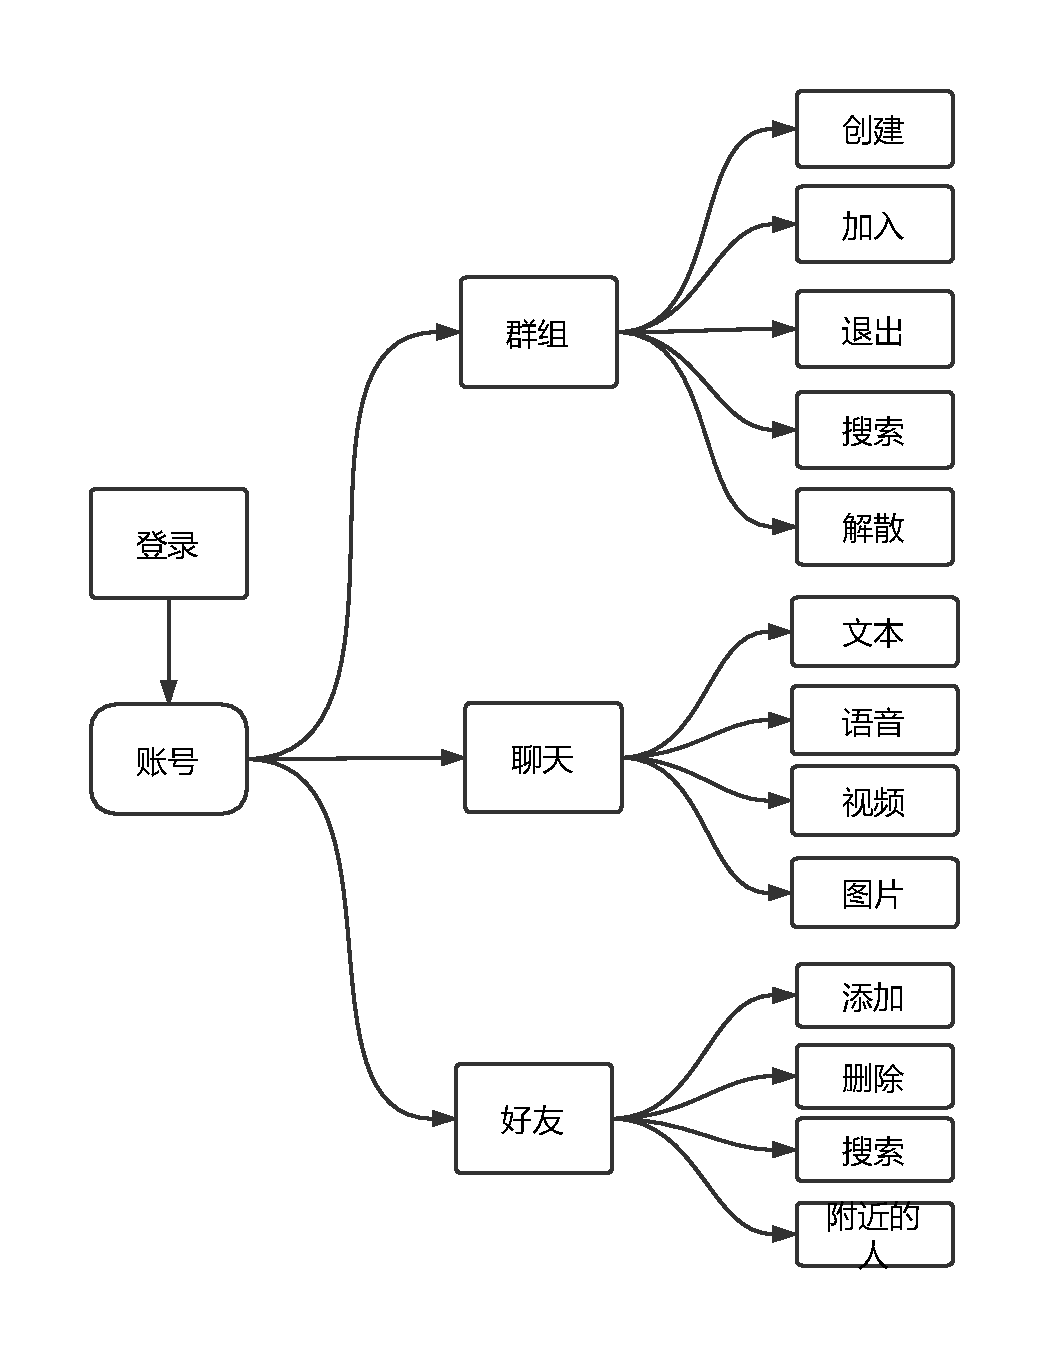
\includegraphics[width=10cm]{function}
	\caption{功能图} \label{fig:function}
\end{figure}

\section{性能需求}
% <If there are performance requirements, state them here and explain their rationale, to help the developers understand the intent and make suitable design choices. Specifies the timing relationships for real time systems. Such requirements should be made as specific as possible. >

% 如果有性能方面的需求,在这里列出并解释他们的原理。以帮助开发者理解意图以做出正确的设计选择。在实时系统中的时序关系。保证需求尽可能的详细而精确。
% \subsection{性能需求1}
% Describes the statically and dynamically quantized requirements on the software (or the interaction between user and the software)
% Static quantized requirement could include:
% A. Maximum number of terminal supported.
% B. Maximum number of users that can use the software at the same time.
% C. Maximum number of files and records to be processed
% D. Maximum size of  tables and files
% Dynamically quantized requirements could include:
% A. Specific duration of normal value and peak value of workload (e.g., one hour)
% B. Number of event and task and data volume to be processed 
% All these requirements should be described by measurable term, for example, saying "95% of the events should be processed in 1 second", instead of saying "the operator need not wait for the business to complete."
% Note: The quantized constraint of a detailed requirement should be described in the subsection of the detailed requirement.
% 本子章节应从整体上描述静态和动态的量化的对软件(或人与软件交互)的需求。
% 
% 静态的量化需求可能包括:
% 
% A. 支持的终端数目。
% 
% B. 支持的同时使用的用户数目。
% 
% C.处理的文件和记录的数目。
% 
% D.表和文件的大小。
% 
% 动态的量化需求可能包括:
% 
% A. 在正常和峰值工作量条件下特定时间段(如一小时)
% 
% B. 处理的事务和任务的数目以及数据量。
% 
% 所有的这些需求应以可测量的术语进行描述,例如所有的操作应在1秒内被处理完成,而不是描述成操作员不必等待操作的完成。
% 
% 注意: 用于一个具体功能的量化限制通常在该功能的处理子章节中描述。

\subsection{实时性需求}

系统应采用推送技术实现聊天消息的实时性。如 android 客户端可以使用 google 或小米等的推送平台,web app可以使用 websocket 长连接。

\subsection{并发性需求}

服务端应采用一定的技术实现高并发,保证在用户数量较大时仍能正常运行。
要求服务器至少能同时支持10000个客户端同时在线。

\section{外部接口需求}
\subsection{用户接口}
% <The interface of the system with the User and vice versa should be explained in detail. >
% 
% 详细描述系统与用户之间的接口
% 
% This section should include:
% A. Features that must be supported by the software for eachman-machine interface. For example, if the user operates from a display terminal, then the following should be included:
% 		Screen format required
% 		Page layout and content of report and menu
% 		Timing sequence for input and output
% 		Usage of some functional key combinations
% B. Every aspect about the use of the system's user interface. It could be a list that shows the user what should do and what should not do.  For example, an option of overlong or overshort message. . And same as other requirements, these requirements should be easily verified. For example, saying "A level 4 typist can finish function X in Z minutes after a one-hour training." instead of "A typist can finish function X"	
% 
% 这应描述下述内容:
% 
% A. 对每种人机界面,软件所必须支持的特性。例如,如果系统用户通过一个显示终端进行操作,那么应包含下述内容:
% 要求的屏幕格式
% 页面规划及报告或菜单的内容
% 输入和输出的相关时序
% 一些组合功能键的用法
% 
% B. 与系统用户接口使用相关的所有方面。这可能只是一个简单的关于系统怎样展示给用户而该做什么和不该做什么的列表。例如提供关于长或短错误消息选项。和所有其它需求一样,这些需求也应能被检验,例如,四级打字员经一小时的培训后能在Z分钟内完成功能X,而不是一个打字员能完成功能X。


\subsubsection{登录界面}

\begin{figure}[h]
	\centering
	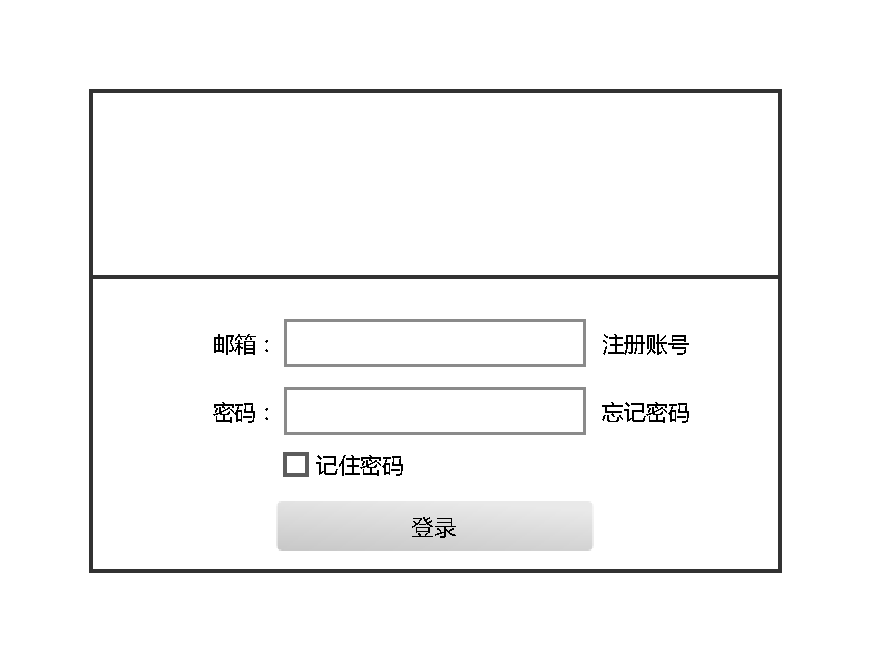
\includegraphics[width=13cm]{login_ui}
	\caption{登录界面} \label{fig:login_ui}
\end{figure}


如图 3.1。
输入邮箱密码登陆,可选择记住密码,右侧有注册账号和忘记密码的按钮。
界面上方放置banner图片,增加美观。

\clearpage
\subsubsection{主界面}
\begin{figure}[h]
	\centering
	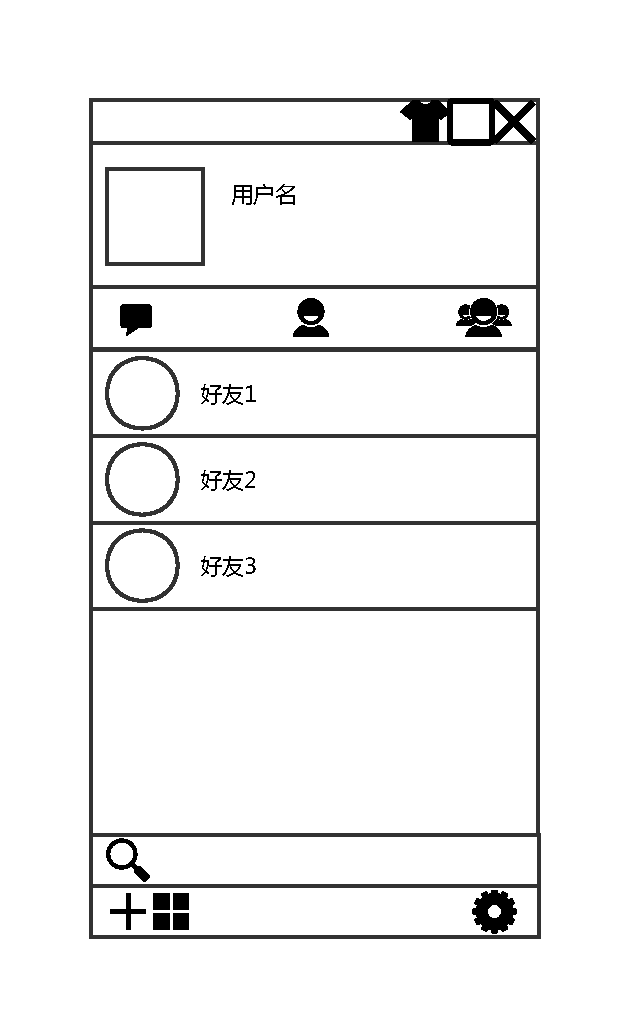
\includegraphics[width=10cm]{main_ui}
	\caption{主界面} \label{fig:main_ui}
\end{figure}

如图 3.2。
最上方显示自己的头像和用户名。
中间有三个标签页,从左到右分别是会话,好友和群组。
下方有一个搜索框,可用于搜索已添加的好友。
最下方的三个按钮的功能分别是添加新好友,菜单和设置。

\clearpage
\subsubsection{聊天界面}
\begin{figure}[h]
	\centering
	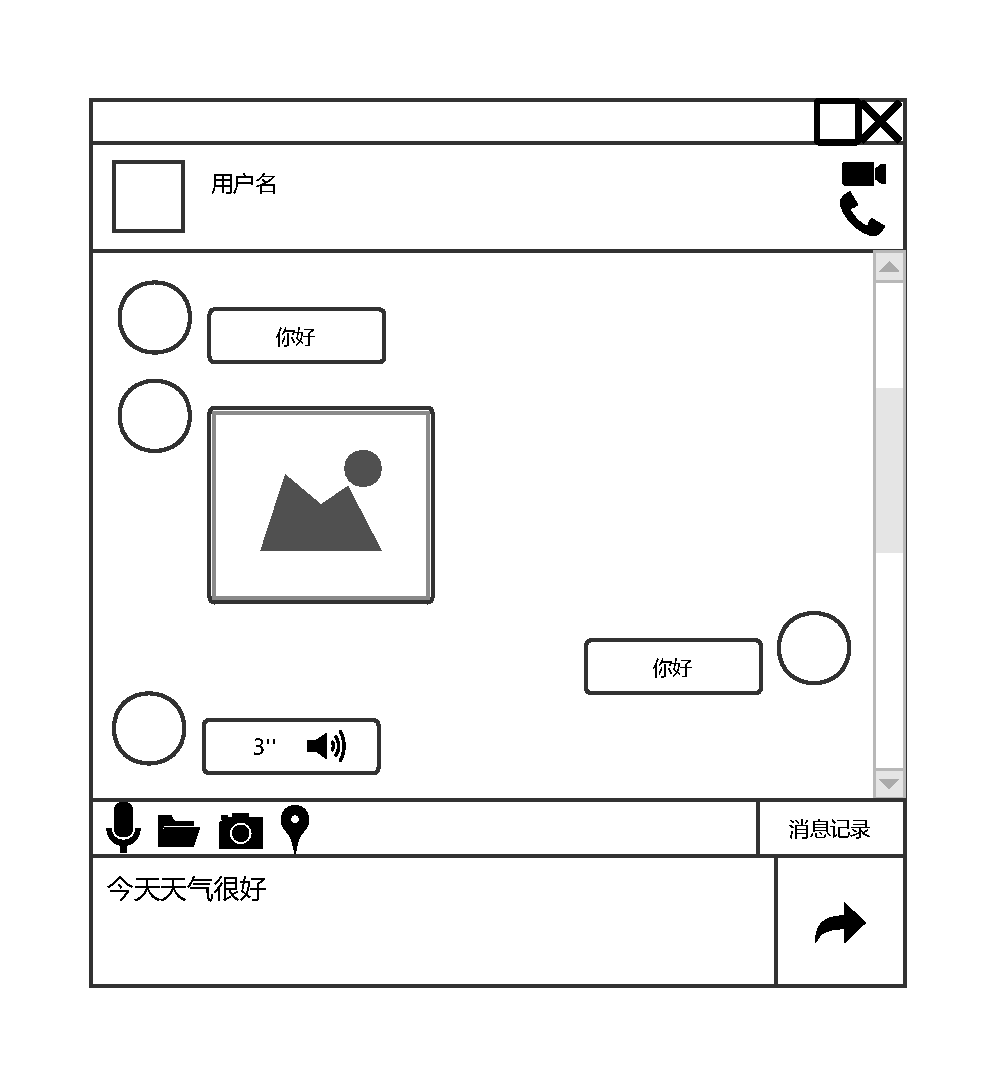
\includegraphics[width=10cm]{chat_ui}
	\caption{聊天界面} \label{fig:chat_ui}
\end{figure}


如图 3.3。
最上方显示对方的头像和用户名(或群的头像和群名),左侧可以开启视频或语音聊天。
中间为消息显示区,消息放在气泡中显示,自己的消息在右侧,其他人的在左侧。
最下方为文本输入框,左侧为发送按钮。
输入框上方为工具栏,可以用于发送图片和语音消息,可以查看聊天记录。

\subsubsection{用户搜索界面}
\begin{figure}[h]
	\centering
	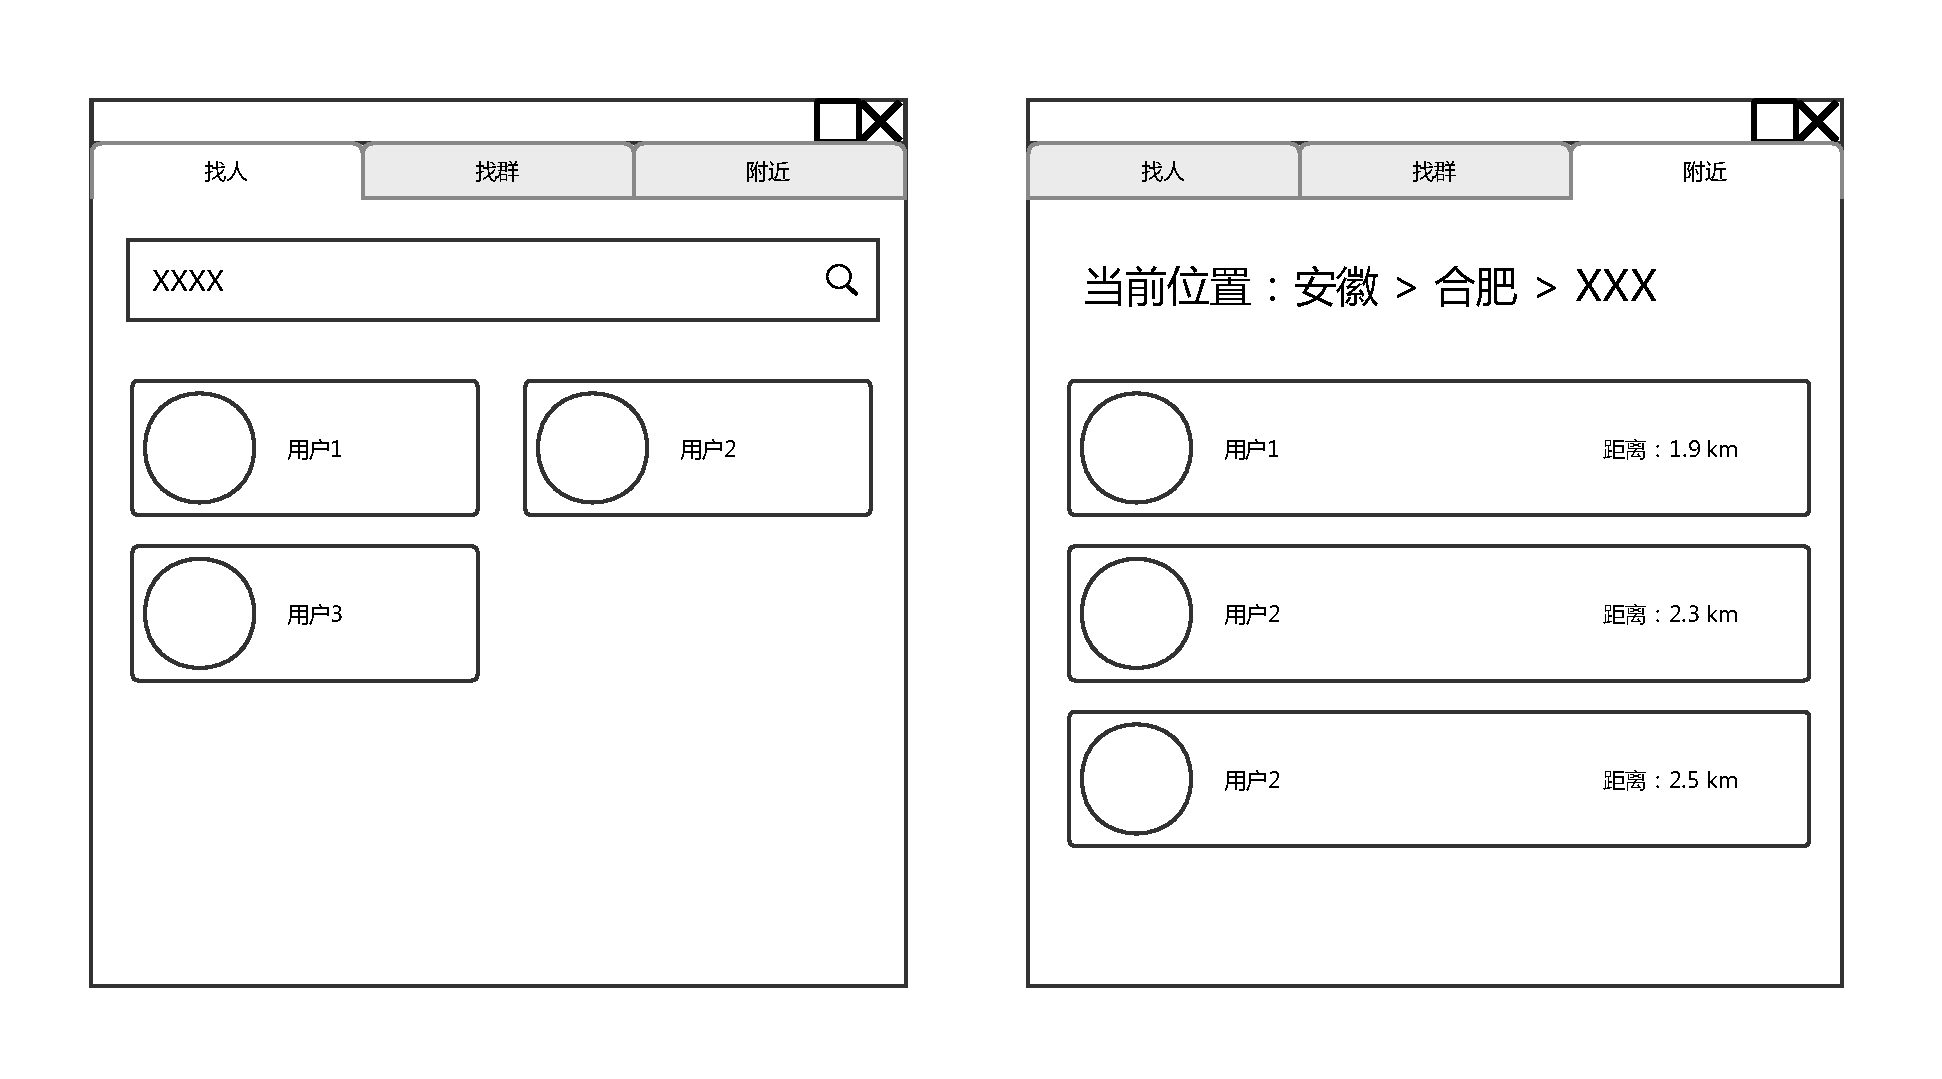
\includegraphics[width=10cm]{search_friend_ui}
	\caption{用户搜索界面} \label{fig:search_friend_ui}
\end{figure}

如图 3.4。
共三个标签页可用于搜人,搜群,附近。
找人,找群标签页在搜索框输入内容后显示结果。
附近标签页显示了当前位置和附近的用户以及估计的距离。
点击用户弹出用户信息界面

\begin{figure}[ht]
	\centering
	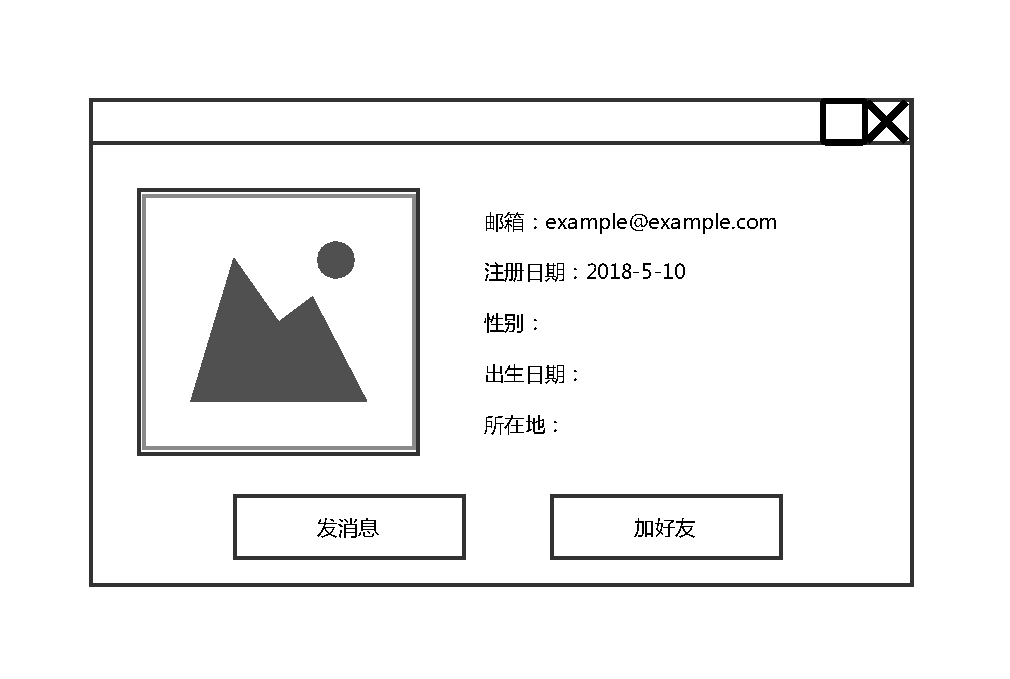
\includegraphics[width=15cm]{userinfo_ui}
	\caption{用户信息界面} \label{fig:userinfo_ui}
\end{figure}


\subsection{软件接口}
% <The interface with other system/modules/projects should be explained in detail. >
% 
% 详细描述与其他系统 /模块 /项目之间的接口
% 
% Describes how to use the other (required) software products. (such as data management system, operation system, or algorithm tools package), and the interfaces to other application systems (such as interfaces between the protocol process system and the database management system )
% For each required software product, following information should be provided:
% A. Name
% B. Mnemonic symbol
% C. Version number
% D. Source
% For each interface, this section should:
% A. Discuss the objective of the required software.
% B. Define the interfaces by content and format of message/function. If the interfaces have been clearly described in other documents, it is not necessary to describe in detail here. But the reference of those documents should be given.
% 
% 在此应描述如何使用其它(必需的)软件产品(例如,数据管理系统,操作系统,或算法工具包),以及与其它应用系统的接口(例如,协议处理系统和数据库管理系统之间的接口)。
% 
% 对每个必需的软件产品,应提供下列信息:
% A.	名字
% B.	助记符
% C.	版本号
% D.	来源
% 
% 对每个接口,本部分应:
% 
% A .	讨论与本软件产品相关的接口软件的目的。
% 
% B.	按消息/函数内容和格式定义接口。如果接口已在其它文档中很清楚地描述,就没有必要在这儿进行详细描述,但需说明应参考的文档。

% ython version > 3.5
% mysql version > 5.7

\subsection{硬件接口}
% <The interface with other hardware components should be explained in detail. >
% 
% 详细描述与硬件的接口
% 
% Describes the logical features of the interface between the software and hardware components, including the equipment supported and how the equipment and protocol is supported. 
% 
% Defines the interfaces according to the content and format of the software/hardware protocol. If the interfaces have been clearly described in other documents, it is not necessary to describe in detail here. But the reference of those documents should be given.
% 
% 在此描述软件产品和系统硬件组件之间接口的逻辑特征,也包括支持哪些设备、怎样支持这些设备和协议等。
%  
% 按软/硬件协议内容和格式定义接口。如果接口已在其它文档中很清楚地描述,就没有必要在这儿进行详细描述,但需说明应参考的文档。

部分平台的客户端需要使用录音设备获取音频输入,使用摄像设备获取视频输入,使用定位设备获取位置信息。

详细硬件接口设计见设计文档。

\subsection{通讯接口}
% <This should specify the various interfaces to communications such as local network protocols, etc.>
% 
% 详细描述通讯接口,如本地网络协议等。
% 
% Defines the interfaces according to the content and format of the message/function. If the interfaces have been clearly described in other documents, it is not necessary to describe in detail here. But the reference of those documents should be given.
% 
% 按消息/函数内容和格式定义接口。如果接口已在其它文档中很清楚地描述,就没有必要在这儿进行详细描述,但需说明应参考的文档。

客户端需要通过互联网和服务端通信,会使用到 Socket 通信和 HTTP 协议。

详细的通信接口设计见设计文档。
\chapter{总体设计约束}
% <Describe any items or issues that will limit the options available to the developers. >

% 描述可能限制开发人员选择的事项。
 
\section{标准符合性}
下面列出了在各种约束中所提及的国际标准、规范:
\begin{itemize}
    \item PEP 8 标准\\
    \url{https://www.python.org/dev/peps/pep-0008/}
    \item OAuth 2.0 授权标准\\
    \url{https://oauth.net/2/}
\end{itemize}

\section{硬件约束}
% <This subsection could include Requirements for the software to operate inside various hardware constraints, such as timing constraints, memory constraints etc.)

% 本节包括软件在不同的硬件平台运行的需求,如时间相关的约束,内存方面的约束等。

对于 x86 桌面平台客户端,
要求安装包小于 30MB,
安装所需空间小于 150MB(不包括数据文件),
运行所需内存小于 200MB,
保证低配置电脑也能正常运行。

对于移动 Android 平台客户端,
要求安装包小于 20MB,
安装所需空间小于 150MB,
运行所需内存小于 300MB(Android平台的应用相对x86平台,会占用更多的内存),
保证低配置手机也能正常运行。

对于 x86 平台服务端,
要求安装所需空间小于 500MB,
运行所需内存小于 1GB。

\section{兼容性约束}
为使产品能够在主流的硬件/软件平台上正确地运行,产品需要满足以下约束要求:
\begin{itemize}
    \item Linux平台下的客户端要支持 Ubuntu,Debian,Centos,Arch 等主流发行版
    \item Windows平台下的客户端需支持 Windows 7 及更高
    \item Android 平台下的客户端需支持到安卓 4.4 及以上
    \item Web app 需支持 Chrome,Firefox,IE11(或更高版本) 等主流浏览器。
    \end{itemize}

\section{技术限制}
% <This subsection could include limitations on the use of specific technologies, interfaces, databases, parallel operations; communications protocols; design conventions or programming standards. >

% 本节包括对使用特定技术的限制,包括接口,数据库,并行操作,通讯协议,设计约定,编程规范等。

数据库和第三方组件应尽可能选用开源产品,便于定制修改。

\begin{itemize}
    \item \textbf{数据库}\\
    考虑到服务的用户数量较为小众,以及本产品的开源、非营利性政策,选用免费的MySQL作为数据库。
    \item \textbf{服务端开发框架}\\
    考虑到开发周期较短,Web应用需求变化较大等因素,我们选用适合快速开发的Django Framework作为服务端的开发框架。
    \item \textbf{并行计算框架}\\
    对于程序中可能需要并行处理的部分,我们采用广泛使用的MPI并行框架来编写代码。
    \item \textbf{编码规范}\\
    开发过程中,应严格遵守Python代码所推荐遵循的PEP8规范。

\end{itemize}
\chapter{软件质量特性}

% <Specify any additional quality characteristics for the project that will be important to either the customers or the developers. Some to consider are: adaptability, availability, correctness, flexibility, interoperability, maintainability, portability, reliability, reusability, robustness, testability, and usability. Write these to be specific, quantitative, and verifiable when possible. At the least, clarify the relative preferences for various attributes, such as ease of use over ease of learning.

% 详细说明项目任何其他的质量特性。该特性对客户和开发者都非常重要。考虑的方面包括:适应性,可用性,正确性,灵活性,交互工作能力,可维护性,可移植性,可靠性,可重用性,鲁棒性,可测试性和可用性等。定量的详细描述这些特性,尽可能的可验证。对不同属性之间的重要性加以阐述,如:易用性比易学性更重要。

% <Please use the below sub-section for each attributes separately. You can copy the section for additional attributes. >

% 每一个属性单独使用一个小节描述,可根据需要进行增减,如增加可维护性小节等。

\section{扩展性与可维护性}
在开发阶段,应做到高度模块化,尽量使单模块内聚,模块间解耦合。模块依赖于抽象的政策,再辅以各种不同的机制或者说一系列接口,政策的具体实现建立于对各种已有机制的组合使用之上。如此开发并配置软件可以更好地支持软件的进化,模块化与分离的政策与机制有利于在出现新的需求时对软件进行快速精准的更改以适应。

从动态运行角度来说,为增强软件的鲁棒性和智能,软件实现时会有特别的模块监督各种接口异常并详尽记录异常信息,以及采取自适应方式从异常信息中学习,然后反馈关键的信息,和做一定程度的异常处理。对于不同的运行环境或系统约束,本产品会以科学的方式进行大量的适配调试,在适应各种已经环境的同时,也保留能快速扩展适应新环境的能力。

\section{可用性}
该即时通讯系统在使用上不应设计得有任何门槛,用户不必花大量的时间和精力来学习和使用已经高度集成化的功能,只需要按照直观的、傻瓜式的UI排布导引,顺应自己的直觉进入相应的模块,便能对其所提供的功能一目了然。使用相应的功能也不需要用户做太多配置,简简单单的点击就能达到用户的通讯目的和相关的一系列小需求。本产品到用户手中开始使用时,可以基本不需要太多导引就能让用户上手,注册自己的ID,添加目标对象作为自己的好友,和最重要的,编辑信息发送给对象以及自动获取对象的发送信息,由此简单轻松地开始用户与好友的即时交流。

\section{正确性}
本产品应经过多环境长时间严格的测试,保障在环境状态允许下,用户与用户之间的交流内容能够准确无误且快速地送达,或是用户上传的信息如个人资料能完成符合用户要求的更改,搜索方面也将以正确的信息回应用户。环境状态不合适时比如网络不佳的状态下通讯,软件会立刻反馈给用户关键的问题提示,使用户知道问题所在并有办法解决问题。

\section{灵活性}
对于客户端,由于其简单可用,不用考虑复杂扩展功能;而对于服务端,可考虑通过如提供启动参数等方式实现部分功能的参数化配置(如聊天记录的保存期限等参数),用户通过简单的配置文件就能灵活实现不同的复杂功能。同时服务端的功能扩展也部分依赖于参数化配置时参数类型的增加。

% \section{交互工作能力}

% \section{可维护性}

% \section{可移植性}

% \section{可靠性}

% \section{可重用性}

% \section{可测试性}


\chapter{其他需求}
<Any other requirement specified by the customer need to be listed below with appropriate section. This may include Database, Coding requirements, Error handling, Testing requirements etc., Few sample requirements are listed below. Please note, you may remove or add if something is not applicable. >
使用适当的章节,详细说明任何其他客户需求,包括数据库,编码需求,错误处理,测试需求等。下面仅列出了少量样例,你可以删除和增加项目。
\section{数据库}
< This could specify the requirements for any database that is to be developed as part of the project. >
详细说明项目相关的数据库方面的需求。
\section{操作}
<This could specify the normal and special operations required by the user. >
详细说明用户通常的和特殊的操作需求。
\section{本地化}
<Any requirement on multi language operation could be described here. >
描述支持多语种的需求。

\chapter{依赖关系}
% <Explain the internal and external dependency for each requirement (if applicable). >

% 解释每一条需求的内部和外部依赖关系。
\subsection{R.INSTANT.MESSAGE.USERS.001 新用户注册}
\subsubsection{内部依赖}
    创建用户资料信息,依赖功能:R.INSTANT.MESSAGE.USERS.002 变更自己的用户资料。
\subsubsection{外部依赖}
    数据库、服务器、客户端以及网络连接的支持。

\subsection{R.INSTANT.MESSAGE.USERS.002 变更自己的用户资料}
\subsubsection{内部依赖}
    无其他内部功能依赖
\subsubsection{外部依赖}
    数据库、服务器、客户端以及网络连接的支持。

\subsection{R.INSTANT.MESSAGE.USERS.003 使用用户ID来查找用户资料}
\subsubsection{内部依赖}
    无其他内部功能依赖
\subsubsection{外部依赖}
    数据库、服务器、客户端以及网络连接的支持。

\subsection{R.INSTANT.MESSAGE.USERS.004 通过地理位置发现周边的用户}
\subsubsection{内部依赖}
    无其他内部功能依赖
\subsubsection{外部依赖}
\begin{itemize}
    \item 数据库、服务器、客户端以及网络连接的支持。
    \item 客户端所在终端的位置信息硬件的支持
\end{itemize}
\subsection{R.INSTANT.MESSAGE.USERS.005 申请好友}
\subsubsection{内部依赖}
    好友的查找、发现依赖如下两个功能:
    \begin{itemize}
        \item R.INSTANT.MESSAGE.USERS.003 使用用户ID来查找用户资料
        \item R.INSTANT.MESSAGE.USERS.004 通过地理位置发现周边的用户
    \end{itemize}
\subsubsection{外部依赖}
数据库、服务器、客户端以及网络连接的支持。

\subsection{R.INSTANT.MESSAGE.CHAT.001 发送文本消息}
\subsubsection{内部依赖}
    无其他内部功能依赖
\subsubsection{外部依赖}
    数据库、服务器、客户端以及网络连接的支持。操作系统输入法组件的支持。

	
\subsection{R.INSTANT.MESSAGE.CHAT.002 发送语音消息}
\subsubsection{内部依赖}
    无其他内部功能依赖
\subsubsection{外部依赖}
    数据库、服务器、客户端以及网络连接的支持。终端设备录音硬件的支持。

\subsection{R.INSTANT.MESSAGE.CHAT.002 发送图片消息}
\subsubsection{内部依赖}
    客户端应用的图片收藏夹功能的支持。
\subsubsection{外部依赖}
    客户端所在终端的文件系统支持。
    数据库、服务器、客户端以及网络连接的支持

\subsection{R.INSTANT.MESSAGE.CHAT.003 创建聊天群组}
\subsubsection{内部依赖}
    无其他内部功能依赖
\subsubsection{外部依赖}
    数据库、服务器、客户端以及网络连接的支持

\subsection{R.INSTANT.MESSAGE.CHAT.005 邀请用户加入聊天群组}
\subsubsection{内部依赖}
    R.INSTANT.MESSAGE.CHAT.003 创建聊天群组
\subsubsection{外部依赖}
    数据库、服务器、客户端以及网络连接的支持

\subsection{R.INSTANT.MESSAGE.CHAT.006 退出聊天群组}
\subsubsection{内部依赖}
    R.INSTANT.MESSAGE.CHAT.003 创建聊天群组
\subsubsection{外部依赖}
    数据库、服务器、客户端以及网络连接的支持

\subsection{R.INSTANT.MESSAGE.CHAT.007 解散聊天群组}
\subsubsection{内部依赖}
\begin{itemize}
    \item R.INSTANT.MESSAGE.CHAT.003 创建聊天群组
    \item R.INSTANT.MESSAGE.CHAT.006 退出聊天群组(解除每个用户与群组的关系时,需要用到)
\end{itemize}
\subsubsection{外部依赖}
    数据库、服务器、客户端以及网络连接的支持

\chapter{需求分级}
\begin{table}[htbp]
\centering
\caption{需求分级表} \label{tab:classification}
\begin{tabular}{|c|c|c|}
    \hline
    需求ID & 需求名称 & 需求分级 \\
    \hline
    a & b & c \\
    \hline
    a & b & c \\
    \hline
    a & b & c \\
    \hline
    a & b & c \\
    \hline
    a & b & c \\
    \hline
    a & b & c \\
    \hline
    a & b & c \\
    \hline
    a & b & c \\
    \hline
\end{tabular}
\end{table}

Importance of requirements are classified as following:
\begin{enumerate}
\item Mandatory: absolutely essential features, without which the product development will be canceled.
\item Important: unessential features that may affect the viability of the product.
\item Nice to have: desired features, the absence of which will not affect the product viability.
\end{enumerate}

重要性分类如下:
\begin{itemize}
\item 必须的		绝对基本的特性;如果不包含,产品就会被取消。
\item 重要的		不是基本的特性,但这些特性会影响产品的生存能力。
\item 最好有的		期望的特性;但省略一个或多个这样的特性不会影响产品的生存能力
\end{itemize}

\chapter{待确定问题}
\begin{table}[htbp]
\centering
\caption{待确定问题表} \label{tab:tbd_problems}
\begin{tabular}{|c|c|c|c|c|c|c|}
    \hline
    需求ID & 问题描述 & 影响(H/M/L) & 风险 & 责任人 & 解决日期 & 状态(Open/Close) \\
    \hline
    % 啊写不下了。。。
    申请好友 & 拒绝好友申请时不应显式地通知申请者 & L & 无 & 罗炳琨 & 2018-04-28 & Close\\
    \hline
\end{tabular}
\end{table}
%\chapter{Latex使用例子}

\section{图}
\subsection{示例}
\begin{figure}[ht]
\centering

\includegraphics[width=10cm]{ustc_logo_fig}
\caption{测试图片} \label{fig:figure1}
\end{figure}

\subsection{带图注的图}
\begin{figure}[ht]
\centering

\includegraphics[width=10cm]{ustc_logo_fig}
\caption{带图注的图片}\label{fig:noted-figure}
\note{the solid lines represent the time histogram of the spontaneous activities of an old monkey cell(gray) and a young monkey cell (black). The bin-width is 1}
\end{figure}

\section{表格}

\subsection{A Simple Table}
\begin{table}[htbp]
\centering
\caption{这里是表的标题} \label{tab:simpletable}
\begin{tabular}{|c|c|}
    \hline
    a & b \\
    \hline
    c & d \\
    \hline
\end{tabular}
\note{这里是表的注释}
\end{table}

\subsection{长表格}
\begin{longtable}{ccc}
% 首页表头
\caption[长表格演示]{长表格演示} \label{tab:longtable} \\
\toprule[1.5pt]
名称  & 说明 & 备注\\
\midrule[1pt]
\endfirsthead
% 续页表头
\caption[]{长表格演示(续)} \\
\toprule[1.5pt]
名称  & 说明 & 备注 \\
\midrule[1pt]
\endhead
% 首页表尾
\hline
\multicolumn{3}{r}{\small 续下页}
\endfoot
% 续页表尾
\bottomrule[1.5pt]
\endlastfoot

AAAAAAAAAAAA   &   BBBBBBBBBBB   &   CCCCCCCCCCCCCC   \\
AAAAAAAAAAAA   &   BBBBBBBBBBB   &   CCCCCCCCCCCCCC   \\
AAAAAAAAAAAA   &   BBBBBBBBBBB   &   CCCCCCCCCCCCCC   \\
AAAAAAAAAAAA   &   BBBBBBBBBBB   &   CCCCCCCCCCCCCC   \\
AAAAAAAAAAAA   &   BBBBBBBBBBB   &   CCCCCCCCCCCCCC   \\
AAAAAAAAAAAA   &   BBBBBBBBBBB   &   CCCCCCCCCCCCCC   \\
AAAAAAAAAAAA   &   BBBBBBBBBBB   &   CCCCCCCCCCCCCC   \\
AAAAAAAAAAAA   &   BBBBBBBBBBB   &   CCCCCCCCCCCCCC   \\
AAAAAAAAAAAA   &   BBBBBBBBBBB   &   CCCCCCCCCCCCCC   \\
AAAAAAAAAAAA   &   BBBBBBBBBBB   &   CCCCCCCCCCCCCC   \\
AAAAAAAAAAAA   &   BBBBBBBBBBB   &   CCCCCCCCCCCCCC   \\
AAAAAAAAAAAA   &   BBBBBBBBBBB   &   CCCCCCCCCCCCCC   \\
AAAAAAAAAAAA   &   BBBBBBBBBBB   &   CCCCCCCCCCCCCC   \\
AAAAAAAAAAAA   &   BBBBBBBBBBB   &   CCCCCCCCCCCCCC   \\
AAAAAAAAAAAA   &   BBBBBBBBBBB   &   CCCCCCCCCCCCCC   \\
AAAAAAAAAAAA   &   BBBBBBBBBBB   &   CCCCCCCCCCCCCC   \\
AAAAAAAAAAAA   &   BBBBBBBBBBB   &   CCCCCCCCCCCCCC   \\
AAAAAAAAAAAA   &   BBBBBBBBBBB   &   CCCCCCCCCCCCCC   \\
AAAAAAAAAAAA   &   BBBBBBBBBBB   &   CCCCCCCCCCCCCC   \\
AAAAAAAAAAAA   &   BBBBBBBBBBB   &   CCCCCCCCCCCCCC   \\
AAAAAAAAAAAA   &   BBBBBBBBBBB   &   CCCCCCCCCCCCCC   \\
AAAAAAAAAAAA   &   BBBBBBBBBBB   &   CCCCCCCCCCCCCC   \\
AAAAAAAAAAAA   &   BBBBBBBBBBB   &   CCCCCCCCCCCCCC   \\
AAAAAAAAAAAA   &   BBBBBBBBBBB   &   CCCCCCCCCCCCCC   \\
AAAAAAAAAAAA   &   BBBBBBBBBBB   &   CCCCCCCCCCCCCC   \\
AAAAAAAAAAAA   &   BBBBBBBBBBB   &   CCCCCCCCCCCCCC   \\
AAAAAAAAAAAA   &   BBBBBBBBBBB   &   CCCCCCCCCCCCCC   \\
AAAAAAAAAAAA   &   BBBBBBBBBBB   &   CCCCCCCCCCCCCC   \\
AAAAAAAAAAAA   &   BBBBBBBBBBB   &   CCCCCCCCCCCCCC   \\
AAAAAAAAAAAA   &   BBBBBBBBBBB   &   CCCCCCCCCCCCCC   \\
AAAAAAAAAAAA   &   BBBBBBBBBBB   &   CCCCCCCCCCCCCC   \\
AAAAAAAAAAAA   &   BBBBBBBBBBB   &   CCCCCCCCCCCCCC   \\
AAAAAAAAAAAA   &   BBBBBBBBBBB   &   CCCCCCCCCCCCCC   \\
AAAAAAAAAAAA   &   BBBBBBBBBBB   &   CCCCCCCCCCCCCC   \\
AAAAAAAAAAAA   &   BBBBBBBBBBB   &   CCCCCCCCCCCCCC   \\
AAAAAAAAAAAA   &   BBBBBBBBBBB   &   CCCCCCCCCCCCCC   \\
\end{longtable}


\section{算法环境}
模板中使用 \texttt{algorithm2e} 宏包实现算法环境。关于该宏包的具体用法,
请阅读宏包的官方文档。

\begin{algorithm}[htbp]
\SetAlgoLined
\KwData{this text}
\KwResult{how to write algorithm with \LaTeX2e }

initialization\;
\While{not at end of this document}{
    read current\;
    \eIf{understand}{
        go to next section\;
        current section becomes this one\;
    }{
        go back to the beginning of current section\;
    }
}
\caption{算法示例1}
\label{algo:algorithm1}
\end{algorithm}

\IncMargin{1em}
\begin{algorithm}
\SetKwData{Left}{left}\SetKwData{This}{this}\SetKwData{Up}{up}
\SetKwFunction{Union}{Union}\SetKwFunction{FindCompress}{FindCompress}
\SetKwInOut{Input}{input}\SetKwInOut{Output}{output}

\Input{A bitmap $Im$ of size $w\times l$}
\Output{A partition of the bitmap}
\BlankLine
\emph{special treatment of the first line}\;
\For{$i\leftarrow 2$ \KwTo $l$}{
    \emph{special treatment of the first element of line $i$}\;
    \For{$j\leftarrow 2$ \KwTo $w$}{\label{forins}
        \Left$\leftarrow$ \FindCompress{$Im[i,j-1]$}\;
        \Up$\leftarrow$ \FindCompress{$Im[i-1,]$}\;
        \This$\leftarrow$ \FindCompress{$Im[i,j]$}\;
        \If(\tcp*[h]{O(\Left,\This)==1}){\Left compatible with \This}{\label{lt}
            \lIf{\Left $<$ \This}{\Union{\Left,\This}}
            \lElse{\Union{\This,\Left}}
        }
        \If(\tcp*[f]{O(\Up,\This)==1}){\Up compatible with \This}{\label{ut}
        \lIf{\Up $<$ \This}{\Union{\Up,\This}}
        \tcp{\This is put under \Up to keep tree as flat as possible}\label{cmt}
        \lElse{\Union{\This,\Up}}\tcp*[h]{\This linked to \Up}\label{lelse}
        }
    }
    \lForEach{element $e$ of the line $i$}{\FindCompress{p}}
}
\caption{算法示例2}\label{algo_disjdecomp}
\label{alog:algorithm2}
\end{algorithm}\DecMargin{1em}


\section{代码环境}
模板中使用 \texttt{listings} 宏包实现代码环境。详细用法见宏包的官方说明文档。

以下是代码示例,可以在文中任意位置引用\autoref{first-code} 。
\begin{lstlisting}[language=C, caption=示例代码, label={code:first-code}]
#include <stdio.h>

int main( )
{
    printf("hello, world\n");
    return 0;
}
\end{lstlisting}




\section{引用文献标注}

\subsection{著者-出版年制标注法}

\noindent
\verb|\citestyle{ustcauthoryear}|
\citestyle{ustcauthoryear}

\noindent
\begin{tabular}{l@{\quad$\Rightarrow$\quad}l}
  \verb|\cite{knuth86a}| & \cite{knuth86a}\\
  \verb|\citet{knuth86a}| & \citet{knuth86a}\\
  \verb|\citet[chap.~2]{knuth86a}| & \citet[chap.~2]{knuth86a}\\[0.5ex]
  \verb|\citep{knuth86a}| & \citep{knuth86a}\\
  \verb|\citep[chap.~2]{knuth86a}| & \citep[chap.~2]{knuth86a}\\
  \verb|\citep[see][]{knuth86a}| & \citep[see][]{knuth86a}\\
  \verb|\citep[see][chap.~2]{knuth86a}| & \citep[see][chap.~2]{knuth86a}\\[0.5ex]
  \verb|\citet*{knuth86a}| & \citet*{knuth86a}\\
  \verb|\citep*{knuth86a}| & \citep*{knuth86a}\\
\end{tabular}

\noindent
\begin{tabular}{l@{\quad$\Rightarrow$\quad}l}
  \verb|\citet{knuth86a,tlc2}| & \citet{knuth86a,tlc2}\\
  \verb|\citep{knuth86a,tlc2}| & \citep{knuth86a,tlc2}\\
  \verb|\cite{knuth86a,knuth84}| & \cite{knuth86a,knuth84}\\
  \verb|\citet{knuth86a,knuth84}| & \citet{knuth86a,knuth84}\\
  \verb|\citep{knuth86a,knuth84}| & \citep{knuth86a,knuth84}\\
\end{tabular}

\subsection{顺序编码制标注法}

\noindent
\verb|\citestyle{ustcnumerical}|
\citestyle{ustcnumerical}

\noindent
\begin{tabular}{l@{\quad$\Rightarrow$\quad}l}
  \verb|\cite{knuth86a}| & \cite{knuth86a}\\
  \verb|\citet{knuth86a}| & \citet{knuth86a}\\
  \verb|\citet[chap.~2]{knuth86a}| & \citet[chap.~2]{knuth86a}\\[0.5ex]
  \verb|\citep{knuth86a}| & \citep{knuth86a}\\
  \verb|\citep[chap.~2]{knuth86a}| & \citep[chap.~2]{knuth86a}\\
  \verb|\citep[see][]{knuth86a}| & \citep[see][]{knuth86a}\\
  \verb|\citep[see][chap.~2]{knuth86a}| & \citep[see][chap.~2]{knuth86a}\\[0.5ex]
  \verb|\citet*{knuth86a}| & \citet*{knuth86a}\\
  \verb|\citep*{knuth86a}| & \citep*{knuth86a}\\
\end{tabular}

\noindent
\begin{tabular}{l@{\quad$\Rightarrow$\quad}l}
  \verb|\citet{knuth86a,tlc2}| & \citet{knuth86a,tlc2}\\
  \verb|\citep{knuth86a,tlc2}| & \citep{knuth86a,tlc2}\\
  \verb|\cite{knuth86a,knuth84}| & \cite{knuth86a,knuth84}\\
  \verb|\citet{knuth86a,knuth84}| & \citet{knuth86a,knuth84}\\
  \verb|\citep{knuth86a,knuth84}| & \citep{knuth86a,knuth84}\\
  \verb|\cite{knuth86a,knuth84,tlc2}| & \cite{knuth86a,knuth84,tlc2}\\
\end{tabular}

\subsection{其他形式的标注}

\noindent
\begin{tabular}{l@{\quad$\Rightarrow$\quad}l}
  \verb|\citealt{tlc2}| & \citealt{tlc2}\\
  \verb|\citealt*{tlc2}| & \citealt*{tlc2}\\
  \verb|\citealp{tlc2}| & \citealp{tlc2}\\
  \verb|\citealp*{tlc2}| & \citealp*{tlc2}\\
  \verb|\citealp{tlc2,knuth86a}| & \citealp{tlc2,knuth86a}\\
  \verb|\citealp[pg.~32]{tlc2}| & \citealp[pg.~32]{tlc2}\\
  \verb|\citenum{tlc2}| & \citenum{tlc2}\\
  \verb|\citetext{priv.\ comm.}| & \citetext{priv.\ comm.}\\
\end{tabular}

\noindent
\begin{tabular}{l@{\quad$\Rightarrow$\quad}l}
  \verb|\citeauthor{tlc2}| & \citeauthor{tlc2}\\
  \verb|\citeauthor*{tlc2}| & \citeauthor*{tlc2}\\
  \verb|\citeyear{tlc2}| & \citeyear{tlc2}\\
  \verb|\citeyearpar{tlc2}| & \citeyearpar{tlc2}\\
\end{tabular}

\bibliography{bib/tex}

\appendix
\chapter{可行性分析结果}
Describe the feasibility analysis results on allocated requirements.

描述对分配需求的可行性分析结果。

\chapter{需求建模 }
\section{数据流图}

    \textbf{注}:对于即时通讯系统,对数据的主要操作是传递数据、分发数据,而不存在独立出来的处理数据的过程。故数据流图的内容实为不多,仅用顶层数据流图足以展示全面,故0层、1层数据流图未再考虑。
\subsection{顶层数据流图}
% <Draw the Top-level DFD here>

% 在这里画出顶层数据流图

\begin{figure}[ht]
    \centering
    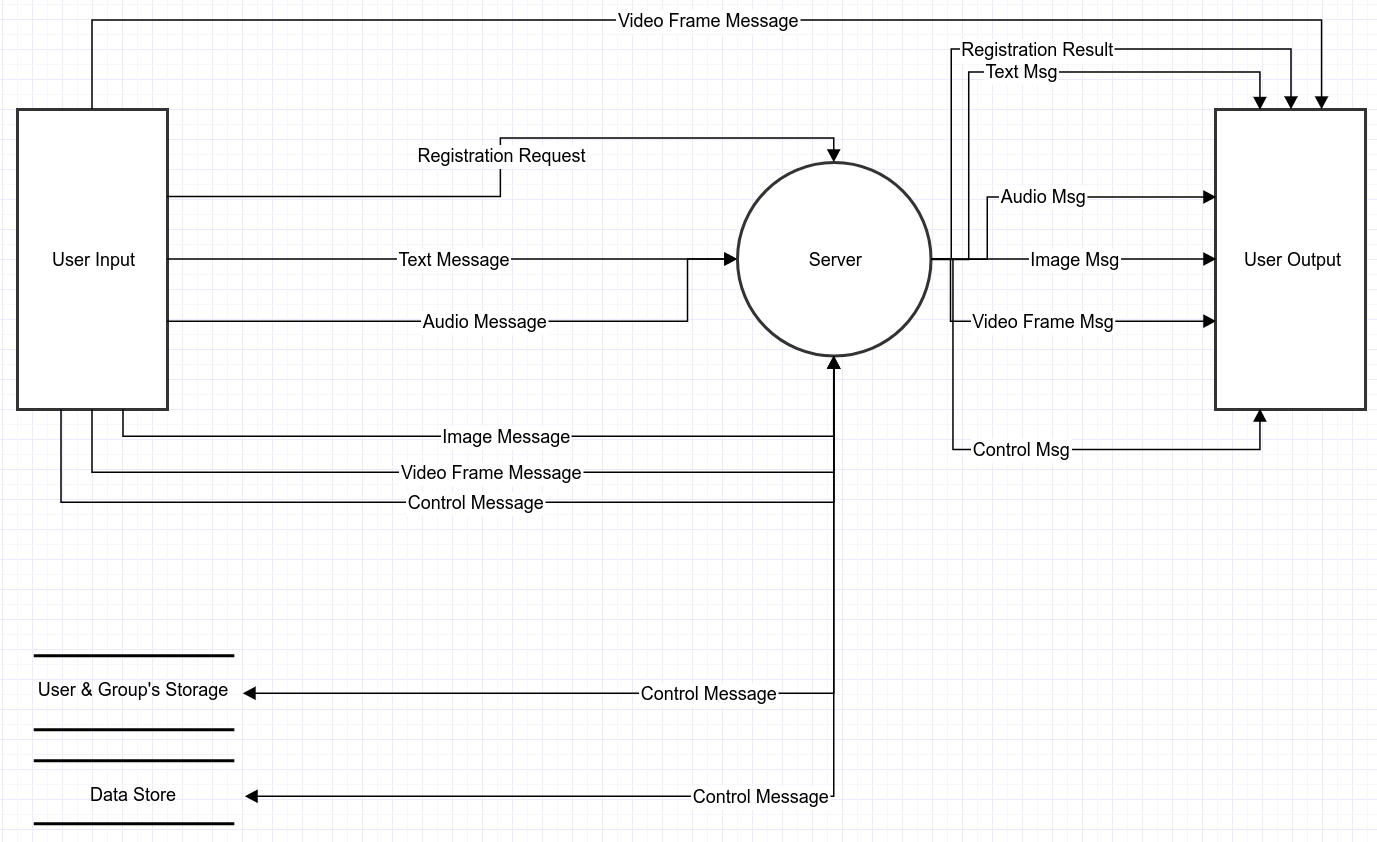
\includegraphics[width=15cm]{data_flow_diagram_high.png}
    \caption{顶层数据流图}\label{fig:figure1}
    
    \end{figure}

% \subsection{层数据流图}
% <Draw the Level-0 DFD here>

% 在这里画出0层数据流图

% \subsection{层数据流图}
% <Draw the Level-1 DFD here>

% 在这里画出1层数据流图

\section{数据字典}
\subsection{数据流说明}
\subsubsection{Registration Request 注册请求信息}
% <Title of  the data flow should accord with the one in data flow diagram, and the Data description notions should be used.  >

% 与数据流图中的名称一致,采用数据描述符号说明数据流的内容
这是由新注册用户所发出的注册请求信息,它包含了用户名,密码等基本信息,以及可选的用户资料(User Profile,如头像,性别,出生日期,所在地等)。

\subsubsection{Registration Result 注册结果信息}
这是返回给新注册用户的注册结果,它指出了注册是否成功,以及一串数字,它将作为该用户第二个用户ID。

\subsubsection{Text Message 文本消息}
这是由已登录用户向另一用户或群组所发出的文本消息。

\subsubsection{Audio Message 语音消息}
这是由已登录用户向另一用户或群组所发出的二进制编码的语音消息。

\subsubsection{Image Message 图片消息}
这是由已登录用户向另一用户或群组所发出的二进制编码的图片消息。

\subsubsection{Video Frame Message 视频帧消息}
这是由已登录用户在进行视频聊天时,不断发出的视频帧消息。\\
注:数据流图中存在两条视频帧消息的数据流,这表示视频帧可能会经过产品服务器的转发,也可能会直接从客户端由UDP协议传输到另一客户端。具体的选择会与当时的网络环境有关。

\subsubsection{Control Message 控制消息}
此类数据流包含多种功能的消息:如添加好友的确认消息、创建群组的命令,以及各种在产品实现中会用到的同步消息。
该类数据流中的有些会作用于另一客户端,有些会作用到服务器的数据库,使得用户、群组在服务器中的存储得以改变。

\subsection{数据存储说明}
\subsubsection{User/Group's Storage 用户和群组存储}
% <Title of  the data flow should accord with the one in data flow diagram, and the Data description notions should be used. The arrangement of the data in data store should also be described.>

% 与数据流图中的名称一致,采用数据描述符号说明数据流的内容,另外还需描述数据排列方式
这块存储区域存储了用户/群组本身的基本信息、用户资料,以及用户与用户之间的好友关系、用户与群组之间的关联。

\subsubsection{Data Store 其他数据存储}
这块存储区域存储了聊天过程中需要保存到云端的数据,如一定期限内的聊天记录。

\subsection{加工说明}
\subsubsection{Server 服务器处理模块}
% <Use natural language, Decision table/Decision tree and Pseudocode to describe how to process the data flow>

% 采用自然语言,判断表/判断树,伪码的形式描述对数据流进行处理的过程
加工各种消息的模块在实现中会十分繁杂,在此将它简化成单一的模块。

\begin{itemize}
    \item \textbf{注册请求(Registration Request)的处理}\\
    服务器会再次验证注册数据的合法性,这是为了防止恶意人员使用产品的API未经客户端的检查而定制自己的请求。\\
    当完成检查后,将输出(Registration Result)发送至用户。
    \item \textbf{各类用户会话消息(文本消息、语音)的处理}\\
    服务器会再次验证消息的完整性、鉴别真实性(通常由消息中的某些字段来鉴别),以及大小是否合适,这也是为了防止恶意人员使用爬虫,通过产品的API,未经客户端的检查而定制自己的请求。\\
    当完成检查后,执行一些必要的序列化操作,将数据以合适的格式发送到目标用户/群组。
    \item \textbf{各类控制消息的处理}\\
    服务器会鉴别控制消息的真实性,如果真实有效,则执行相应操作,将输出的更改存入相应的数据库。
\end{itemize}




\end{document}
